\ifx\wholebook\relax \else

\documentclass{article}

%
% loading packages
%

\RequirePackage{ifpdf}
\RequirePackage{ifxetex}

%
%
\ifpdf
  \RequirePackage[pdftex,%
       bookmarksnumbered,%
              colorlinks,%
          linkcolor=blue,%
              hyperindex,%
        plainpages=false,%
       pdfstartview=FitH]{hyperref}
\else\ifxetex
  \RequirePackage[bookmarksnumbered,%
               colorlinks,%
           linkcolor=blue,%
               hyperindex,%
         plainpages=false,%
        pdfstartview=FitH]{hyperref}
\else
  \RequirePackage[dvipdfm,%
        bookmarksnumbered,%
               colorlinks,%
           linkcolor=blue,%
               hyperindex,%
         plainpages=false,%
        pdfstartview=FitH]{hyperref}
\fi\fi
%\usepackage{hyperref}

% other packages
%--------------------------------------------------------------------------
\usepackage{graphicx, color}
\usepackage{wrapfig}
\usepackage{subfig}
\usepackage{multicol}
\usepackage{tikz}
\usetikzlibrary{matrix,positioning,shapes}
\usetikzlibrary{patterns}

\usepackage{amsmath, amsthm, amssymb} % for math
\usepackage{exercise} % for exercise
\usepackage{import} % for nested input

%
% for programming
%
\usepackage{verbatim}
\usepackage{fancyvrb}
\usepackage{listings}
%\usepackage{algorithmic} %old version; we can use algorithmicx instead
%\usepackage[plain]{algorithm} %remove rule (horizontal line on top/below the algorithm
\usepackage{algorithm} %to remove rules change to \usepackage[plain]{algorithm}
%\usepackage{algorithm2e}
\usepackage[noend]{algpseudocode} %for pseudo code, include algorithmicsx automatically
\usepackage{appendix}
\usepackage{makeidx} % for index support
\usepackage{titlesec}
\usepackage{epigraph}

\usepackage[cm-default]{fontspec}
\usepackage{xunicode}
%\usepackage{fontenc}
\usepackage{textcomp}
\usepackage{url}

% detect and select Chinese font
% ------------------------------
% fc-list :lang=zh    % list all Chinese fonts
% fc-list :mono       % list all mono fonts
% fc-cache            % refresh cache to load new installed fonts
\def\macmainfont{STSong}  % Under Mac OS X
\def\macmonofont{Monaco}
\def\winmainfont{SimSun} % Under Windows
\def\winmonofont{Consolas}
\def\linuxmainfont{WenQuanYi Micro Hei} % Under Linux
\def\linuxmainfont{Courier}

\suppressfontnotfounderror1 % Avoid setting exit code (error level) to break make process
\count255=\interactionmode
\batchmode

% main font
\let\mainft=\macmainfont
\font\thefont="\mainft"\space at 10pt
\ifx\thefont\nullfont
  \let\mainft=\winmainfont
  \font\thefont="\mainft"\space at 10pt
  \ifx\the\nullfont
    \let\mainft=\linuxmainfont
    \font\thefont="\mainft"\space at 10pt
    \ifx\the\nullfont
      \errorstopmode
      \errmessage{no suitable Chinese main font found}
    \fi
  \fi
\fi

% mono font
\let\monoft=\macmonofont
\font\thefont="\monoft"\space at 10pt
\ifx\thefont\nullfont
  \let\monoft=\winmonofont
  \font\thefont="\monoft"\space at 10pt
  \ifx\the\nullfont
    \let\monoft=\linuxmonofont
    \font\thefont="\monoft"\space at 10pt
    \ifx\the\nullfont
      \errorstopmode
      \errmessage{no suitable mono font found}
    \fi
  \fi
\fi

\interactionmode=\count255

\setmainfont[Mapping=tex-text]{\mainft}
\setmonofont[Scale=MatchLowercase]{\monoft}   % 英文等宽字体

\XeTeXlinebreaklocale "zh"  % to solve the line breaking issue
\XeTeXlinebreakskip = 0pt plus 1pt minus 0.1pt

\titleformat{\paragraph}
{\normalfont\normalsize\bfseries}{\theparagraph}{1em}{}
\titlespacing*{\paragraph}
{0pt}{3.25ex plus 1ex minus .2ex}{1.5ex plus .2ex}

\lstdefinelanguage{Smalltalk}{
  morekeywords={self,super,true,false,nil,thisContext}, % This is overkill
  morestring=[d]',
  morecomment=[s]{"}{"},
  alsoletter={\#:},
  escapechar={!},
  literate=
    {BANG}{!}1
    {UNDERSCORE}{\_}1
    {\\st}{Smalltalk}9 % convenience -- in case \st occurs in code
    % {'}{{\textquotesingle}}1 % replaced by upquote=true in \lstset
    {_}{{$\leftarrow$}}1
    {>>>}{{\sep}}1
    {^}{{$\uparrow$}}1
    {~}{{$\sim$}}1
    {-}{{\sf -\hspace{-0.13em}-}}1  % the goal is to make - the same width as +
    %{+}{\raisebox{0.08ex}{+}}1		% and to raise + off the baseline to match -
    {-->}{{\quad$\longrightarrow$\quad}}3
	, % Don't forget the comma at the end!
  tabsize=2
}[keywords,comments,strings]

% for literate Haskell code
\lstdefinestyle{Haskell}{
  flexiblecolumns=false,
  basewidth={0.5em,0.45em},
  morecomment=[l]--,
  literate={+}{{$+$}}1 {/}{{$/$}}1 {*}{{$*$}}1 {=}{{$=$}}1
           {>}{{$>$}}1 {<}{{$<$}}1 {\\}{{$\lambda$}}1
           {\\\\}{{\char`\\\char`\\}}1
           {->}{{$\rightarrow$}}2 {>=}{{$\geq$}}2 {<-}{{$\leftarrow$}}2
           {<=}{{$\leq$}}2 {=>}{{$\Rightarrow$}}2
           {\ .}{{$\circ$}}2 {\ .\ }{{$\circ$}}2
           {>>}{{>>}}2 {>>=}{{>>=}}2
           {|}{{$\mid$}}1
}

% "define" Scala
\lstdefinelanguage{Scala}{
  morekeywords={abstract,case,catch,class,def,%
    do,else,extends,false,final,finally,%
    for,if,implicit,import,match,mixin,%
    new,null,object,override,package,%
    private,protected,requires,return,sealed,%
    super,this,throw,trait,true,try,%
    type,val,var,while,with,yield},
  otherkeywords={=>,<-,<\%,<:,>:,\#,@},
  sensitive=true,
  morecomment=[l]{//},
  morecomment=[n]{/*}{*/},
  morestring=[b]",
  morestring=[b]',
  morestring=[b]"""
}

\lstloadlanguages{C, C++, Java, Lisp, Haskell, Python, Smalltalk, Scala}

\lstset{
  basicstyle=\small\ttfamily,
  commentstyle=\rmfamily,
  texcl=true,
  showstringspaces = false,
  upquote=true,
  flexiblecolumns=false
}

\newcommand\doubleplus{+\kern-1.3ex+\kern0.8ex}

% ======================================================================

\def\BibTeX{{\rm B\kern-.05em{\sc i\kern-.025em b}\kern-.08em
    T\kern-.1667em\lower.7ex\hbox{E}\kern-.125emX}}

%
% mathematics
%
\newcommand{\be}{\begin{equation}}
\newcommand{\ee}{\end{equation}}
\newcommand{\bmat}[1]{\left( \begin{array}{#1} }
\newcommand{\emat}{\end{array} \right) }
\newcommand{\VEC}[1]{\mbox{\boldmath $#1$}}

% numbered equation array
\newcommand{\bea}{\begin{eqnarray}}
\newcommand{\eea}{\end{eqnarray}}

% equation array not numbered
\newcommand{\bean}{\begin{eqnarray*}}
\newcommand{\eean}{\end{eqnarray*}}

\newtheorem{theorem}{定理}[section]
\newtheorem{lemma}[theorem]{引理}
\newtheorem{proposition}[theorem]{Proposition}
\newtheorem{corollary}[theorem]{Corollary}

% 中文书籍设置
% ====================================
\renewcommand\contentsname{目\ 录}
%\renewcommand\listfigurename{插图目录}
%\renewcommand\listtablename{表格目录}
\renewcommand\figurename{图}
\renewcommand\tablename{表}
\renewcommand\proofname{证明}
\renewcommand\ExerciseName{练习}
%\renewcommand{\algorithmcfname}{算法}

\ifx\wholebook\relax
\renewcommand\bibname{参\ 考\ 文\ 献}                    %book类型
%\newtheorem{Definition}[Theorem]{定义}
\newtheorem{Theorem}{定理}[chapter]
\newtheorem{example}{例题}[chapter]
\else
\renewcommand\refname{参\ 考\ 文\ 献}
\fi

%\setcounter{secnumdepth}{4}
\titleformat{\chapter}
  {\normalfont\bfseries\Large}
  {第\arabic{chapter}章}
  {12pt}{\Large}
%% \titleformat{\subsection}
%%   {\normalfont\bfseries\large}
%%   {\CJKnumber{\arabic{subsection}}、}
%%   {12pt}{\large}
%% \titleformat{\subsubsection}
%%   {\normalfont\bfseries\normalsize}
%%   {\arabic{subsubsection}.}
%%   {12pt}{\normalsize}

%\renewcommand{\baselinestretch}{1.5}                        %文章行间距为1.5倍。

\makeatletter
\newcommand{\verbatimfont}[1]{\renewcommand{\verbatim@font}{\ttfamily#1}}
\makeatother

\setcounter{tocdepth}{4}
\setcounter{secnumdepth}{4}

%\verbatimfont{\footnotesize}


\setcounter{page}{1}

\begin{document}

\title{无穷}

\author{刘新宇
\thanks{{\bfseries 刘新宇} \newline
  Email: liuxinyu95@gmail.com \newline}
  }

\maketitle
\fi

\markboth{无穷}{编程的数学原理}

\ifx\wholebook\relax
\chapter{无穷}
\numberwithin{Exercise}{chapter}
\fi

\epigraph{我明白了,但我不相信。}{——理查德$\cdot$戴得金}

% "I see it, but I don't believe it." -- Richard Dedekind

\begin{wrapfigure}{R}{0.5\textwidth}
 \centering
 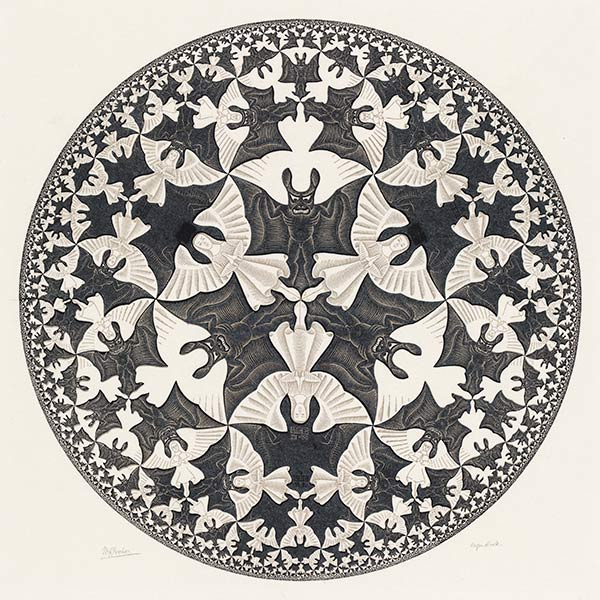
\includegraphics[scale=0.3]{img/circle-limit-IV-1960.eps}
 \captionsetup{labelformat=empty}
 \caption{埃舍尔《圆极限$\cdot$4》(又名天使与恶魔)1960}
 \label{fig:Penrose-triangle}
\end{wrapfigure}

不知在多久以前,我们的祖先仰望星空,面对浩瀚的星河,由衷地发出感叹,我们所在的世界究竟有多大?
作为智慧的生命,我们的思维超越自我,超越地球,超越宇宙,不断思考着无穷的概念。我们的祖先是从具体的事物中抽象出数了的概念。
例如狩猎得到的三头羊,采集得到三个果实,烧制了三个陶罐,进而得到抽象的数字三来代表任何三个东西。起初的数字大小有限,能够满足日常生活、狩猎、劳作。
随着文明的发展,我们开始进行贸易活动,出于记账的要求,所需要的数字逐渐变大。人们发展出种种计数系统,来掌握更大的数字。
终于,我们提出问题:最大的数是什么?对于这个问题,人们采用两种不同的态度。一种认为,这个问题没有意义,在古代,
掌握千百万这样的数已经足够生活中使用了。我们无需了解生活中用不上的大数。例如我们可以认为世界上沙子的数目是无穷的。
在古希腊,一万曾被认为是一个十分巨大的数,人们称它为murias,最终变成了myriad一词,意为“无数”\cite{De-linfini-2018}。无独有偶,佛教中也用“恒河沙数”来表达大到无法计算的数。在大乘佛教经典《金刚经》中,佛陀说:“以七宝满尔所恒河沙数三千大世界,以用布施。”另一种则不这么想,阿基米德,这位古希腊伟大的数学家认为,即使是充满全宇宙的沙子数目,也可以用一个数代表。在阿基米德在他的著作《数沙者》开篇中说:

“格朗王,有人认为沙子的数量是无穷的。我所说的沙子,并不单单地指叙拉古附近和西西里岛其余地方的沙子,还包括地球上所有角落能找到的沙子,无论那里有人还是无人居住。另一些人虽然承认沙子的数量并不是无穷大的,但他们认为,我们不可能写出一个足够大的数,使它在数量上超过地球上全部沙子所代表的数量。如果想象一个和地球体积同样大的沙体,而且要从地球上的大海和谷底算起,知道最高山峰的高度都填满沙子,这些人恐怕就更加肯定,世界上不可能有如此之大的数,可以用来表示堆积起这一巨大沙体所需要的沙子的数量。但是,我将向您证明,通过一系列几何张明——您之后也可以照着做——我命名了一些数字,写在我给宙克西珀的手稿中。其中一些数字不仅超过了以我刚刚描述过的方式填充地球所需要的沙子的数量,甚至超过了填充整个宇宙所需要的沙子数量。”

\begin{figure}[htbp]
%\begin{wrapfigure}{R}{0.4\textwidth}
 \centering
 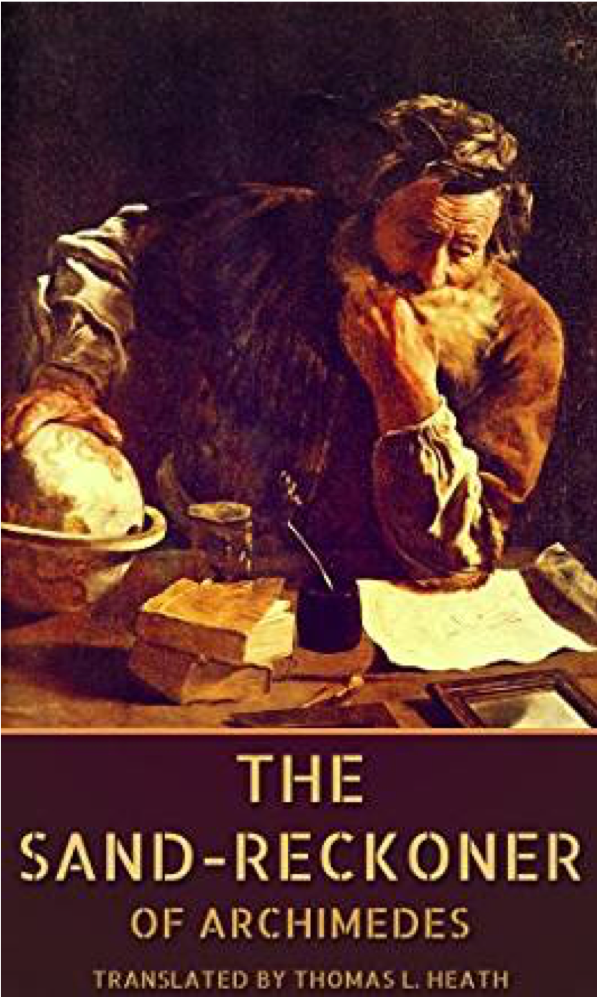
\includegraphics[scale=0.5]{img/Archimedes.eps}
 \captionsetup{labelformat=empty}
 \caption{《数沙者》,封面的阿基米德像是意大利画家多米尼克$\cdot$费蒂1620年创作的。}
 \label{fig:Archimedes}
%\end{wrapfigure}
\end{figure}

阿基米德认为填满宇宙“只”需要$10^{63}$粒沙子。这个宇宙的含义是指恒星天球,大约为两万倍地球的半径。今天我们知道可观测宇宙的尺寸大约为460亿光年,大约包含$3 \times 10^{74}$个原子\footnote{一说为$10^{80}$到$10^{87}$个基本粒子。}。在古希腊的时代,阿基米德的想法无疑是天才的,这几乎是无穷的具体化。我们从语言中,可以看到许多表达大数的单位的词语。例如下表是汉语中的大单位,从“兆”以后,每增加一万倍,就有一个对应的单位。(\cite{Noguchi2007},第31页)

\begin{center}
% for Pinyin tones: \={a}, \'{a}, \v{}, \.{a}
\begin{tabular}{|l|r|l|r|}
\hline
京            & $10^{16}$ & 载            & $10^{44}$ \\
\hline
垓(g\={a}i)   & $10^{20}$ & 极            & $10^{48}$ \\
\hline
秭(z\v{i})    & $10^{24}$ & \textbf{恒河沙}  & $10^{52}$ \\
\hline
穰(r\'{a}ng)  & $10^{28}$ & 阿僧祗(zh\={i})  & $10^{56}$ \\
\hline
沟            & $10^{32}$ & 那由他        & $10^{60}$ \\
\hline
涧            & $10^{36}$ & 不可思议      & $10^{64}$ \\
\hline
正            & $10^{40}$ & 无量大数      & $10^{68}$ \\
\hline
\end{tabular}
\end{center}

可以看到,汉语中这些大单位词汇,由许多来自佛教。包括恒河沙,它表示1后面跟着52个0。英语中的大单位如下表。从一开始,每增加一千倍就有一个对应的单位。这种万进位和千进位的不同,也是文化上的一种差异。

\begin{center}
\begin{tabular}{|l|r|l|r|l|r|}
\hline
thousand & $10^{3}$ & quattuordecillion & $10^{45}$ & octovigintillion & $10^{87}$ \\
\hline
million & $10^{6}$ & quindecillion & $10^{48}$ & novemvigintillion & $10^{90}$ \\
\hline
billion & $10^{9}$ & sexdecillion & $10^{51}$ & trigintillion & $10^{93}$ \\
\hline
trillion  & $10^{12}$ & septdecillion & $10^{54}$ & untrigintillion & $10^{96}$ \\
\hline
quadrillion  & $10^{15}$ & octodecillion & $10^{57}$ & duotrigintillion & $10^{99}$ \\
\hline
quintillion  & $10^{18}$ & novemdecillion & $10^{60}$ & \textbf{googol} & $10^{100}$ \\
\hline
sexillion    & $10^{21}$ & vigintillion & $10^{63}$ & & \\
\hline
septillion   & $10^{24}$ & unvigintillion & $10^{66}$ & & \\
\hline
octillion    & $10^{27}$ & duovigintillion & $10^{69}$ & & \\
\hline
noniliion  & $10^{30}$ & trevigintillion & $10^{72}$ & & \\
\hline
decillion  & $10^{33}$ & quattuorvigintillion & $10^{75}$ & & \\
\hline
undecillion   & $10^{36}$ & quinvigintillion & $10^{78}$ & & \\
\hline
duodecillion  & $10^{39}$ & sexvigintillion & $10^{81}$ & & \\
\hline
tredecillion  & $10^{42}$ & seprvigintillion & $10^{84}$ & & \\
\hline
\end{tabular}
\end{center}

表中最后一个大单位古格尔(googol)是在1920年由9岁的米尔顿$\cdot$西洛塔(Milton Sirotta)想出的名字。这个数字是1后面跟着100个零。著名的互联网公司谷歌的名字就来自它\cite{Wikipedia-Googol}。

超越一切具体大数的无穷是否存在不仅是一个数学问题,还是一个哲学问题。无穷大还直接导致另一个概念——无穷小。古代中国的哲学家庄子在《天下篇》中说:“一尺之棰,日取其半,万世不竭。”,古希腊的哲学家,埃利亚学派的芝诺(Zeno of Elea)提出了著名的四个悖论,它们都与无穷有关。

\begin{figure}[htbp]
%\begin{wrapfigure}{R}{0.3\textwidth}
 \centering
 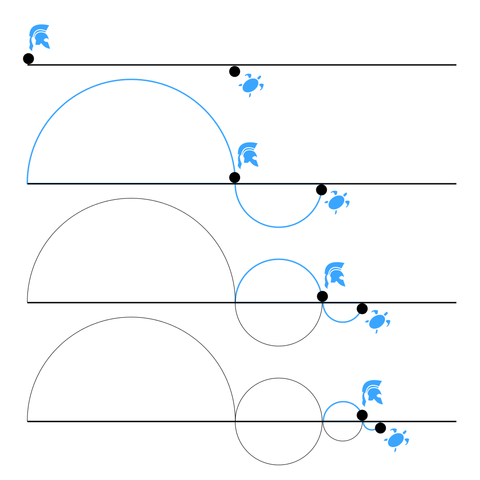
\includegraphics[scale=0.5]{img/Achilles-paradox.eps}
 %\captionsetup{labelformat=empty}
 \caption{阿基里斯与乌龟悖论}
 \label{fig:Achilles-paradox}
%\end{wrapfigure}
\end{figure}

第一个悖论最为人们所津津乐道。名叫阿基里斯与乌龟悖论。阿基里斯是荷马史诗《伊里亚特》中的英雄,以善跑著称。这个悖论说:如果让爬得很慢的乌龟在阿基里斯前面一段路程出发,那么阿基里斯将永远追不上乌龟。这时因为,阿基里斯为了赶上乌龟,必须先到达乌龟的出发点$A$,但当阿基里斯到达$A$点时,乌龟已经在这段时间前进到了$B$点。但当阿基里斯到达$B$点时,乌龟又已经到了前面的$C$点……以此类推,两者间的距离虽然越来越近,但阿基里斯永远落在乌龟的后面而追不上乌龟。如图\ref{fig:Achilles-paradox}所示。但是这与我们生活中的常识是不相符的。这个悖论的推理是如此让人信服,以至于千百年来吸引了无数学者的研究。刘易斯$\cdot$卡罗尔(Lewis Carrol)、侯世达(Douglas Hofstadter)甚至拿乌龟和阿基里斯作为文学作品中的主人公。

第二个悖论叫做“二分悖论”。这个悖论说,如果阿基里斯想从$A$到$B$,那么他必须先走到$1/2$的位置。同样在此之前,他必须要到达$1/4$的位置。而为了到达这一位置,他必须先到达$1/8$的位置……以此类推。由于这样的中点有无限多个,阿基里斯永远也也无法到达目的。芝诺的这个悖论实际上说明了运动根本无法发生。

\begin{figure}[htbp]
%\begin{wrapfigure}{R}{0.3\textwidth}
 \centering
 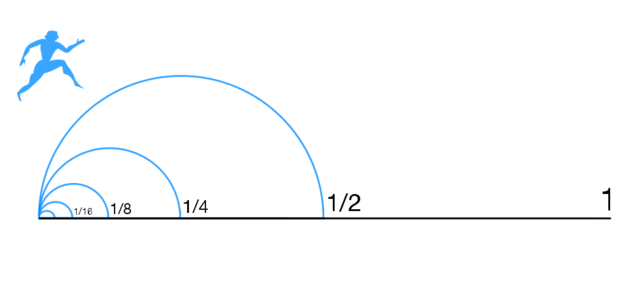
\includegraphics[scale=0.5]{img/Dichotomy-paradox.eps}
 %\captionsetup{labelformat=empty}
 \caption{二分悖论}
 \label{fig:Dichotomy-paradox}
%\end{wrapfigure}
\end{figure}

第三个悖论叫做“飞矢不动悖论”,它从另一个角度描述无穷导致运动无法发生。芝诺指出,任何物体待在相同的位置都不叫运动,可是飞行的箭矢在任一时刻不也是待在一个地方么?这样说来,自然飞失也是不动的。如果说前两个悖论是由于分割空间导致的,则这个悖论是由对时间的分割导致的。

%\begin{figure}[htbp]
\begin{wrapfigure}{R}{0.3\textwidth}
 \centering
 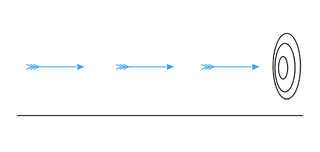
\includegraphics[scale=0.25]{img/Arrow-paradox.eps}
 \captionsetup{labelformat=empty}
 \caption{飞失不动悖论}
 \label{fig:Dichotomy-paradox}
\end{wrapfigure}
%\end{figure}


\begin{wrapfigure}{L}{0.3\textwidth}
 \centering
 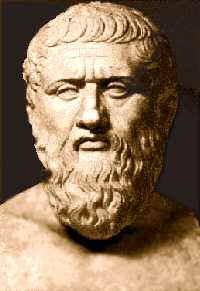
\includegraphics[scale=0.6]{img/Zeno.eps}
 \captionsetup{labelformat=empty}
 \caption{芝诺,约490BC - 425BC}
 \label{fig:Zeno-of-Elea}
\end{wrapfigure}

芝诺的生平

阿基米德的穷竭法

实用观点的发展,微积分,无穷的符号∞

潜无穷的例子,流与惰性求值

流的范畴论解释

实无穷的思考

希尔伯特旅馆

一一对应与无穷集合

康托尔与戴得金

利用(可数)无穷定义斐波那契数列和哈明数列

可数无穷和不可数无穷——实数集

对角线证明

戴得金分割

连续统假设

无穷与艺术

非欧几何

\begin{wrapfigure}{L}{0.4\textwidth}
 \centering
 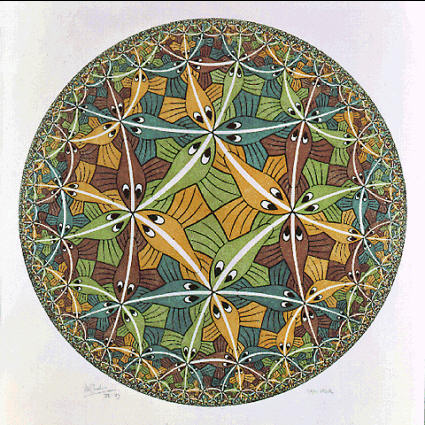
\includegraphics[scale=1.0]{img/circle-limit-III-1959.eps}
 \captionsetup{labelformat=empty}
 \caption{埃舍尔《圆极限$\cdot$3》1959}
 \label{fig:Penrose-triangle}
\end{wrapfigure}

% Mathematicians aren't satisfied because they know there are no solutions up to four million or four billion, they really want to know that there are no solutions up to infinity. -- Andrew Wiles

\ifx\wholebook\relax \else
\begin{thebibliography}{99}

\bibitem{De-linfini-2018}
[法] 让-皮埃尔$\cdot$卢米涅,马克$\cdot$拉雪茨-雷 著,孙展 译. 从无穷开始——科学的困惑与疆界. 人民邮电出版社. 2018. ISBN: 9787115479198

\bibitem{Noguchi2007}
[日] 野口哲也 著,刘慧 韩丽红 译. 数学原来可以这样学. 湖南人民出版社. 2014. ISBN: 9787556100897
% Tetsunori Noguchi. SUGAKUTEKI SENSE GA MINITUKU RENSHUCHO.

\bibitem{Wikipedia-Googol}
Wikipedia. ``Googol''. \url{https://en.wikipedia.org/wiki/Googol}

\end{thebibliography}

\expandafter\enddocument
%\end{document}

\fi
